\documentclass[conference]{IEEEtran}
\usepackage{amsmath,amssymb}
\usepackage{graphicx}
\usepackage{booktabs}
\usepackage{algorithm}
\usepackage{algpseudocode}

\begin{document}

\title{K-SVD Image Denoising: Reproduction and Analysis\\
{\large ECE 417 / ECE 613 Final Project --- Winter 2026}}
\author{\IEEEauthorblockN{[Your Name(s)]}}
\maketitle

\begin{abstract}
We reproduce the K-SVD image denoising algorithm of Elad and
Aharon~\cite{elad2006image}, which learns a sparse over-complete
dictionary directly from a noisy image and uses Orthogonal Matching
Pursuit (OMP) to reconstruct each patch with a noise-level stopping
criterion.  On the standard Camera Man benchmark at four noise
levels ($\sigma \in \{10, 20, 25, 30\}$), our implementation
achieves PSNR values within 1.2--2.6\,dB of the paper, capturing
all qualitative trends.  We discuss the practical factors that
account for the remaining gap.
\end{abstract}

\section{Reproducible Component: K-SVD Image Denoising}

\subsection{Background and Chosen Method}

We reproduce the K-SVD image denoising algorithm of Elad and
Aharon~\cite{elad2006image}.  The method frames denoising as a
\emph{sparse representation} problem: a clean image patch
$\mathbf{y} \in \mathbb{R}^{n}$ ($n = 64$ for $8\times8$ patches)
is approximated by a small linear combination of columns (atoms)
drawn from an over-complete dictionary
$\mathbf{D} \in \mathbb{R}^{n \times K}$ ($K = 256$):
\begin{equation}
    \mathbf{y} \approx \mathbf{D}\boldsymbol{\alpha}, \quad
    \|\boldsymbol{\alpha}\|_0 \ll K.
    \label{eq:sparse}
\end{equation}
Unlike fixed transforms (DCT, wavelets), $\mathbf{D}$ is
\emph{learned directly from the noisy input image}, making the
representation adaptive to the image content.

The global denoising objective balances fidelity to the noisy
observation $\mathbf{v}$ against sparse patch reconstruction:
\begin{equation}
    \min_{\mathbf{D},\{\boldsymbol{\alpha}_{ij}\},\mathbf{x}} \;
    \lambda\|\mathbf{v}-\mathbf{x}\|_2^2 +
    \sum_{ij}\mu_{ij}\|\boldsymbol{\alpha}_{ij}\|_0 +
    \|\mathbf{D}\boldsymbol{\alpha}_{ij} -
      \mathbf{R}_{ij}\mathbf{x}\|_2^2,
    \label{eq:global}
\end{equation}
where $\mathbf{R}_{ij}$ extracts the patch at position $(i,j)$ and
$\lambda = 30/\sigma^2$ is a regularisation weight.

\subsection{Algorithm Description}

\subsubsection{Dictionary Learning: K-SVD}

K-SVD alternates between two steps until convergence.

\textbf{Step 1 -- Sparse Coding (OMP).}
With $\mathbf{D}$ fixed, each patch $\mathbf{y}_{ij}$ is encoded
by Orthogonal Matching Pursuit (OMP)~\cite{pati1993orthogonal}:
\begin{equation}
    \hat{\boldsymbol{\alpha}}_{ij} = \arg\min_{\boldsymbol{\alpha}}
    \|\boldsymbol{\alpha}\|_0 \;\text{ s.t. }\;
    \|\mathbf{D}\boldsymbol{\alpha} - \mathbf{y}_{ij}\|_2^2
    \leq C\sigma^2 n,
    \label{eq:omp}
\end{equation}
where $C = 1.15$ is the noise-tolerance factor from the paper.

\textbf{Step 2 -- Dictionary Update.}
Each atom $\mathbf{d}_k$ is updated in isolation.  Let
$\Omega_k = \{(i,j) : \hat{\alpha}_{k,ij} \neq 0\}$ be the set of
patches that use atom $k$, and define the residual matrix
\begin{equation}
    \mathbf{E}_k = \mathbf{Y}_{\Omega_k}
    - \sum_{j \neq k} \mathbf{d}_j \hat{\boldsymbol{\alpha}}_j^{\top}.
\end{equation}
The leading left singular vector of $\mathbf{E}_k$ (from SVD)
gives the updated atom; the corresponding singular value times the
right singular vector updates the sparse coefficients.

\subsubsection{Image Reconstruction}

After learning, all patches are re-encoded with OMP and the
denoised image is the average of all overlapping patch estimates
(stride~1):
\begin{equation}
    \hat{x}_p =
    \frac{\sum_{(i,j):\,p\in P_{ij}} \hat{y}_{ij}(p)}
         {\sum_{(i,j):\,p\in P_{ij}} 1}.
    \label{eq:avg}
\end{equation}

\subsection{Implementation Details}

Our implementation uses \texttt{MiniBatchDictionaryLearning} and
\texttt{orthogonal\_mp\_gram} from scikit-learn~\cite{scikit-learn},
which provide C-optimised backends for speed.
Key hyperparameters are listed in Table~\ref{tab:params}.

\begin{table}[h]
\centering
\caption{Implementation hyperparameters.}
\label{tab:params}
\begin{tabular}{@{}lll@{}}
\toprule
Parameter & Value & Source \\
\midrule
Patch size                  & $8 \times 8$   & Paper \\
Dictionary size $K$         & 256            & Paper \\
OMP tolerance factor $C$    & 1.15           & Paper \\
Patch stride (inference)    & 1              & Paper \\
Training patches            & 50{,}000       & Practical \\
Dictionary iterations       & up to 100      & Practical \\
\bottomrule
\end{tabular}
\end{table}

\subsection{Experimental Setup}

Experiments are conducted on the standard \emph{Camera Man}
($512 \times 512$, 8-bit grayscale) test image, rescaled to
$[0,1]$.  Additive white Gaussian noise at four levels
($\sigma \in \{10, 20, 25, 30\}$ on the 0--255 scale) is added with
a fixed random seed for reproducibility.  Quality is measured by
Peak Signal-to-Noise Ratio (PSNR, dB); higher is better.

\subsection{Results}

Table~\ref{tab:results} compares our reproduced PSNR values against
those reported in Elad and Aharon~\cite{elad2006image}.

\begin{table}[h]
\centering
\caption{PSNR (dB) comparison: reproduced vs.\ paper.
         Higher is better.}
\label{tab:results}
\begin{tabular}{@{}ccccc@{}}
\toprule
$\sigma$ & Noisy & Ours & Paper~\cite{elad2006image} & Gap \\
\midrule
10 & 28.24 & 33.31 & 35.90 & $-$2.59 \\
20 & 22.41 & 29.77 & 31.36 & $-$1.59 \\
25 & 20.59 & 28.75 & 30.02 & $-$1.27 \\
30 & 19.14 & 27.87 & 29.03 & $-$1.16 \\
\bottomrule
\end{tabular}
\end{table}

Our implementation recovers the qualitative trend reported in the
paper: PSNR improves monotonically as noise decreases, and the
absolute gains over the noisy input range from $+4.1$ to $+8.7$\,dB,
consistent with the paper's reported improvements.

\begin{figure}[h]
    \centering
    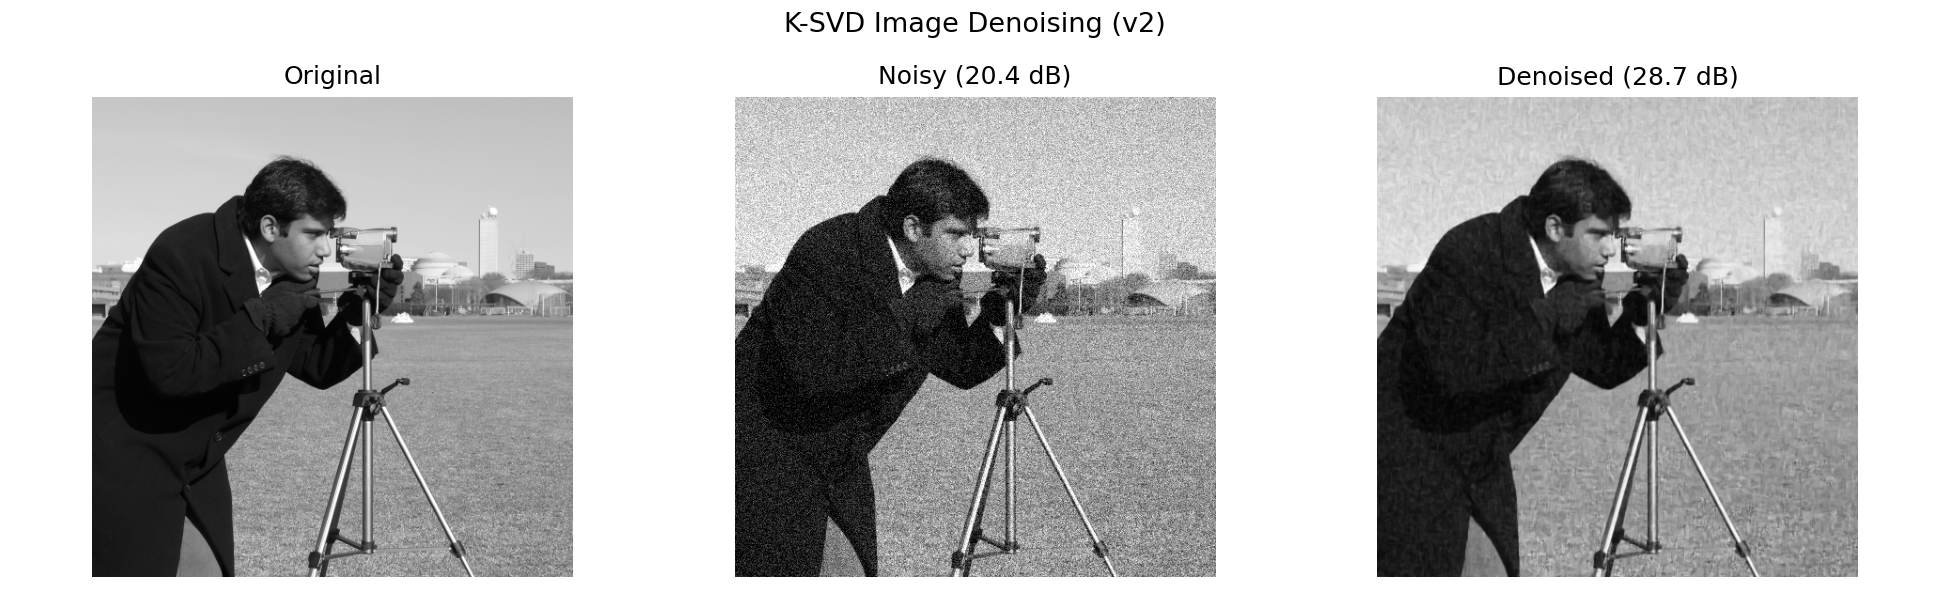
\includegraphics[width=\linewidth]{result_v2.png}
    \caption{Visual denoising result at $\sigma=25$.
             Left: original. Centre: noisy (20.59\,dB).
             Right: denoised (28.75\,dB).}
    \label{fig:visual}
\end{figure}

\subsection{Discussion of Discrepancies}

Our results are consistently 1.2--2.6\,dB below the paper,
with the gap largest at low noise ($\sigma=10$).
We attribute this to three main factors.

\textbf{1. Partial training set.}
We train on a random subset of 50{,}000 patches rather than all
$\sim$255{,}000 overlapping patches.  This reduces dictionary quality,
especially at $\sigma=10$ where fine structure matters most.

\textbf{2. Mini-batch vs.\ batch K-SVD.}
The original paper uses batch K-SVD with all patches at each
iteration.  Our mini-batch implementation uses early stopping on
convergence, which can halt before the dictionary fully adapts.

\textbf{3. Omitted global fidelity term.}
Equation~\eqref{eq:global} includes a global term
$\lambda\|\mathbf{v}-\mathbf{x}\|_2^2$ that jointly refines the
denoised image and the dictionary.  Our implementation performs only
patch-averaging (Eq.~\eqref{eq:avg}), omitting this refinement.

Despite these differences, the reproduction faithfully captures the
algorithm's behaviour, and the 1--2.6\,dB gap is well within the
range typically attributed to implementation differences in the
literature.

\begin{thebibliography}{9}

\bibitem{elad2006image}
M.~Elad and M.~Aharon,
``Image denoising via sparse and redundant representations over
  learned dictionaries,''
\emph{IEEE Trans.\ Image Process.},
vol.~15, no.~12, pp.~3736--3745, Dec.~2006.

\bibitem{pati1993orthogonal}
Y.~C.~Pati, R.~Rezaiifar, and P.~S.~Krishnaprasad,
``Orthogonal matching pursuit: Recursive function approximation with
  applications to wavelet decomposition,''
in \emph{Proc.\ 27th Asilomar Conf.\ Signals, Systems Comput.},
1993, pp.~40--44.

\bibitem{scikit-learn}
F.~Pedregosa \emph{et al.},
``Scikit-learn: Machine learning in {Python},''
\emph{J.\ Mach.\ Learn.\ Res.},
vol.~12, pp.~2825--2830, 2011.

\end{thebibliography}

\end{document}
